%\subsection{Motivating Environment}

Scotland comprises 1/3rd of the area of Great Britian, though its population is
less than 10\%. It is also home to 790 islands, 95 of which are inhabited with
\textasciitilde 100,000 people. The Scottish Highlands and Islands, where this
work is currently focussed, consist of mountainous terrain stretching along a
400km north to south corridor. Islands are scattered on the West together with
deep lakes and glens penetrating the mainland to the East.  The economy was
traditionally maritime, and nearly all habitation is at sea level or in the
glens.

Fibre in the region has only recently appeared.  Much of the telephone network
in the region was constructed with microwave links. Infrastructure is improving,
though plans terminate at telephone exchanges. Among them, fibre-based
services are rare. In the medium term future, local wireless distribution is the
only feasible technology for adequate bandwidth and quality of service.

Starting in 2008, the Tegola project~\cite{tegola} started to
experiment with technology that would enable communities to build
their own wireless networks.
% This included electrical and mechanical infrastructure as well as radio
% equipment.  It rapidly became clear that volunteer communities or small
% businesses could construct and maintain these networks at a small fraction of
% the cost that a centralized organizaton would charge for a number of reasons:
% first, the cost and time of travel to service the relays in remote areas is
% infinitessimal compared with the cost of a helicopter; second site licences and
% wayleaves can usually be negotiated for free by lightweight agreements; third,
The details of the Tegola, and its dissemination to nearby communities, are
omitted due to space constraints. Relevant to this project is the technology
that emerged. Figure~\ref{fig:mhialairigh}, for example, features the type of
robust, inexpensive relay construction that operates in mountainous region, and
that can be constructed by its residents.

\begin{figure}[h]
\centering
 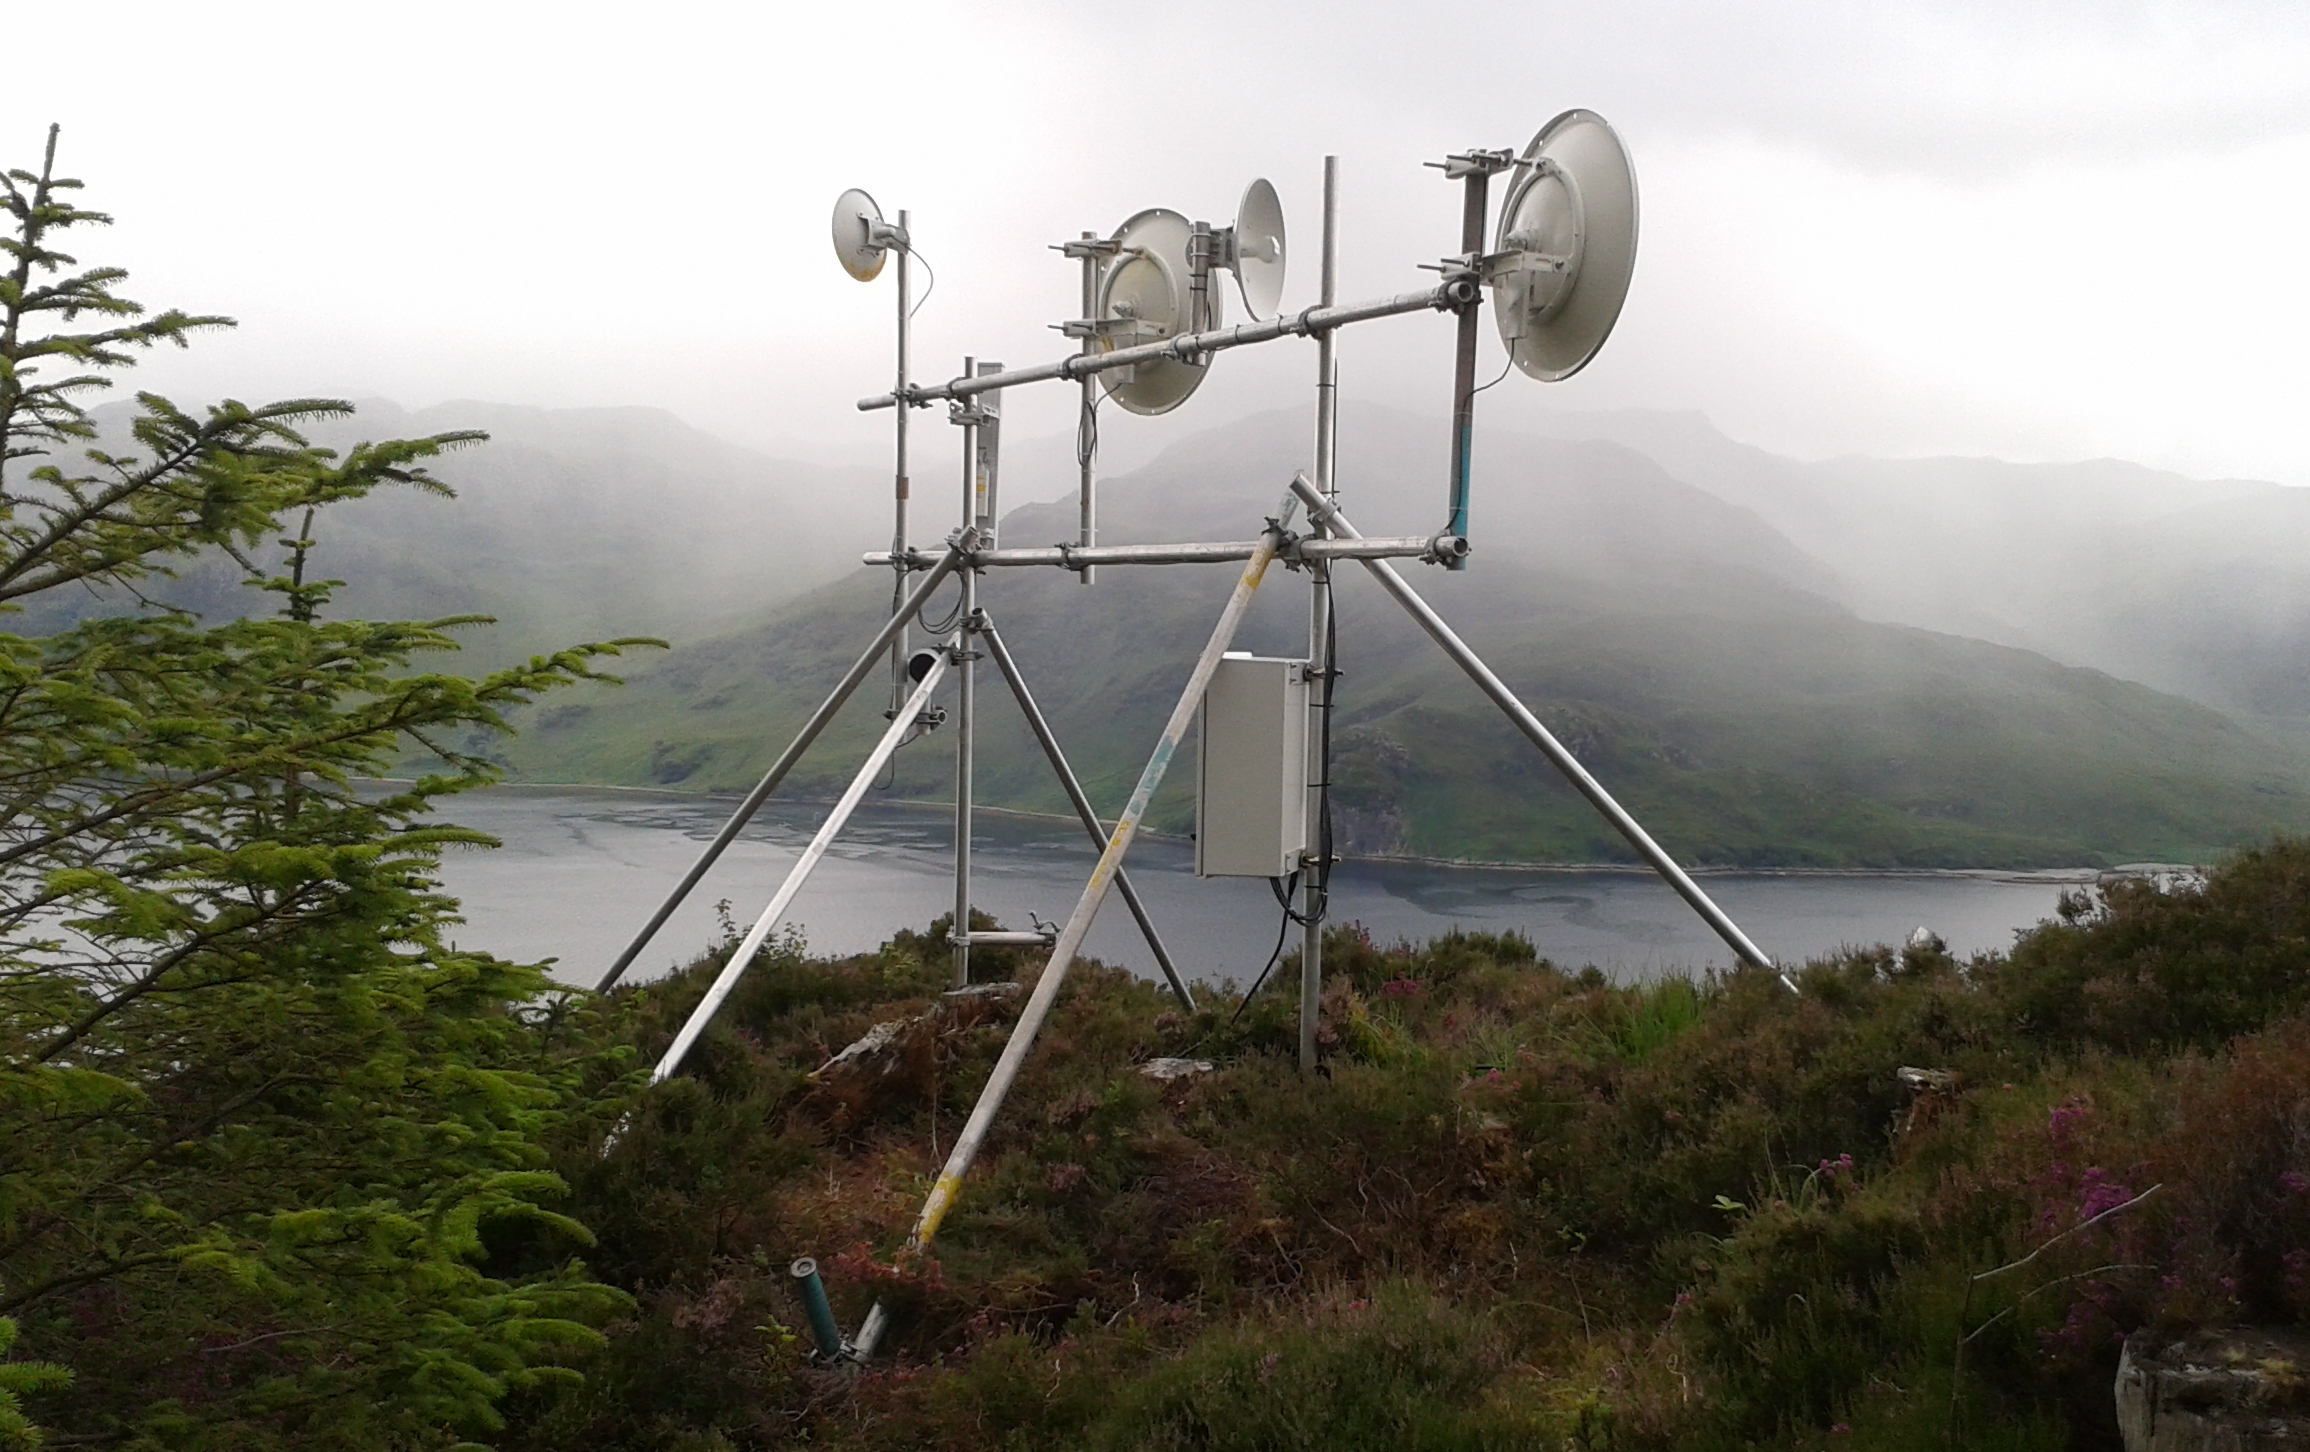
\includegraphics[width=\columnwidth]{figs/mhialairigh-from-behind}
 \caption{A basic relay}
\label{fig:mhialairigh}
\end{figure}

% The ideas were taken up by a number of communities across Scotland
% including those around the Tegola project which extend over 100km of
% the coastline (Fig.~\ref{fig:whixmap}). A typical community would have
% a local distribution network and point-to-point links, often in excess
% of 20km, connected to a set of ADSL lines somewhere near a telephone
% exchange. This was far from ideal, but it was the only affordable
% source of backhaul. Although the communities shared their expertise
% and sometimes their infrastructure, they operated independently.

% Recently, it has become possible to obtain Ethernet services in two
% major towns, but the cost is only reasonable if communities combine
% and buy at wholesale prices.  For this one needs two things: an
% organisational vehicle for the communities act together to achieve
% economies of scale, and a networking infrastructure.

Many communities have since constructed their own local distribution networks
with point-to-point wireless links that can span more than 20km. Expertise is
often shared between them, also infrastructure where feasible, yet they operate
independently. Constrained by availability, they acquire backhaul via ADSL lines
nearby to telephone exchanges. Ethernet services have since emerged in two
larger towns, with wholesale pricing that exceeds the budget of any single
community. A resolution has two components: An organizational vehicle that
combines networks to generate economies of scale, and a supporting network
infrastructure.

% The terrain and the sociology of the Highlands and Island raises some
% important issues for both of these.

We have learned that solutions are complicated by both terrain and by culture.
In particular we note the following observations.
\begin{itemize}%[noitemsep]
\item Social aspects and organization of communities can fail to align with the
  ideal ``electronic'' or networked communities, eg. physical landscape constrains
  connectivity, while social and economic groups can be determined by vehicles for funding.
  % It is relatively easy to bounce signals
  % back and forth across a loch or glen, but extremely hard to carry
  % them over a 1000m high range of mountains. On the other hand
  % social and economic groupings can be determined by the ways in which
  % they obtain funding.%\footnote{Knoydart is an isolated
    %% peninsula (see Fig.~\ref{fig:whixmap})  of which the North and
    %% West coasts are served by a network based on Loch Hourn and the
    %% South coast is served by Loch Nevis.  Contrast this with the Sleat
    %% peninsula which could, rationally,  be split into three sections,
    %% served by Loch Hourn, Loch Nevis and Eigg, but is run
    %% independently as a single entity with three connections to the
    %% rest of the world.}.
\item Local network infrastructure is non-uniform and varies in complexity.
  % between communities structure their networks in various ways, and the
  % complexity varies from a single hub and spoke toplogy to a network
  % with a dozen links including redundant paths.
  % between relays for redundancy.
% \item Many adjacent communities have successfully duplicated the local
%   access network model. Together they cover a significantly large,
%   contiguous geographical area.
\item Communities that share network resources generally do so in a
  non-systematic or ad-hoc manner.
\end{itemize}

%% Stimulated in part by developments in the Highlands and Islands,
%% communities in the Scottish Borders South of Edinburgh started to
%% develop similar networks.  While the terrain is also mountainous, the
%% communities are within 40km of Edinburgh where fibre services are
%% available.  However these are only affordable if the communities
%% combine to purchase bandwidth at scale. To this end a community
%% interest company, HUBS, was established whose members are the
%% communities itself.  In addition to backhaul, HUBS provides technical
%% help and other services.  It is anticipated that HUBS will extend its
%% reach to serve the West Coast and achieve further economies of scale,
%% for example in the puchase of transit.

\subsection{HUBS C.I.C.}\label{subsec:hubs}

In response to the local environment and absence of affordable
backhaul, the Universities of Edinburgh and Stirling launched
HUBS. HUBS is a not-for-profit transit provider whose members are the
community networks that it serves.  HUBS is also a co-operative where
the networks that subscribe also become members. It is the culmination
of collaborations between Universities with communities in the West
Highlands, and later with community networks in the South Scotland.

The need for RemIX-like functionality arose soon after launch. Two of
the subscriber networks took advantage of mutual proximity to
collaborate on an operational basis. Equipment management and
troubleshooting tasks, for example, were shared. Their desire to keep
the details internal was complicated by the fact that their only
interconnection was mediated by HUBS. Circuits were hand-crafted
between them, and demonstrated the benefits of bilateral agreements
between HUBS members. However, while effective, hand-crafted circuits
would fail to scale.

HUBS bridges gaps in backhaul affordability. It has also revealed the
benefits emerge when remote and rural networks are able to act
collectively in the wholesale telecommunications market, and present a
uniform interface to their upstream transit provider. However, a
transit-only solution prohibits autonomous arrangements between
members unmediated at the IP layer. From this need the RemIX
architecture emerges.


% %% Relevant HUBS History
% In 2012-2013 a collaboration took place between the University of
% Stirling and three community networks on the West Coast. They were
% physically neighbouring but were not connected to each other; there
% was no way for them to share resources or provide mutual operational
% support. One had a fast connection via \ac{UHI} but the others could
% make no use of it. Though they were each constructed using similar
% equipment, they were logically organised very differently: one was
% simply a flat layer-2 network, another used static IP routing and the
% third used dynamic routing. It was observed~\cite{waites2014ripe} that
% to connect them together without disturbing their internal structure
% could best be done using \ac{BGP}. And so it was done, to good effect.
%
% At the same time, a similar cluster of community networks was emerging
% in the rural areas to the South of Edinburgh. The proximity to a major
% urban centre presented an opportunity to create a specialist not for
% profit transit provider to cater to their needs. The arrangement up
% North with \ac{UHI} was good but somewhat limiting as institutional
% networks are seldom designed for transit at their periphery. In order
% to have more buying power, the networks wanted to treat with upstream
% providers collectively but no commercial providers had suitable
% products or offerings. So the networks of the South were organised
% together along similar lines as their counterparts in the West
% Highlands, but now with a transit provider of their own. This transit
% provider was called HUBS and it operates \ac{AS} 60241.
%
% Over the course of time, two of the networks in South Scotland began
% to collaborate closely on an operational basis, sharing management and
% troubleshooting tasks for each other's equipment. But their only
% interconnection was mediated by HUBS, which was a hinderance --- they
% did not wish to leak internal details to HUBS but did wish to do so
% between themselves. An ad-hoc solution involving hand-crafted circuits
% was found, but it was obvious that though the capability to have
% bilateral arrangements was very useful, this approach would not scale.
% When financing was obtained to build an upgraded backbone to connect
% the networks on the West Coast --- who now numbered a dozen --- the
% design described herein was developed. The remote networks would be
% able to act collectively in the wholesale telecommunications market,
% present a uniform interface to their upstream transit provider, and
% yet be able to autonomously make arrangements amongst themselves
% unmediated at the IP layer.
